% submitted, the released final. Compile: pdflatex pipeline.tex
\documentclass[tikz,border=3pt]{standalone}
\usepackage[T1]{fontenc}
\usepackage{lmodern}
\usetikzlibrary{arrows.meta,positioning}
\definecolor{pixel}{HTML}{245C83}
\definecolor{select}{HTML}{A34F24}
\definecolor{train}{HTML}{727980}
\begin{document}
\sffamily\footnotesize
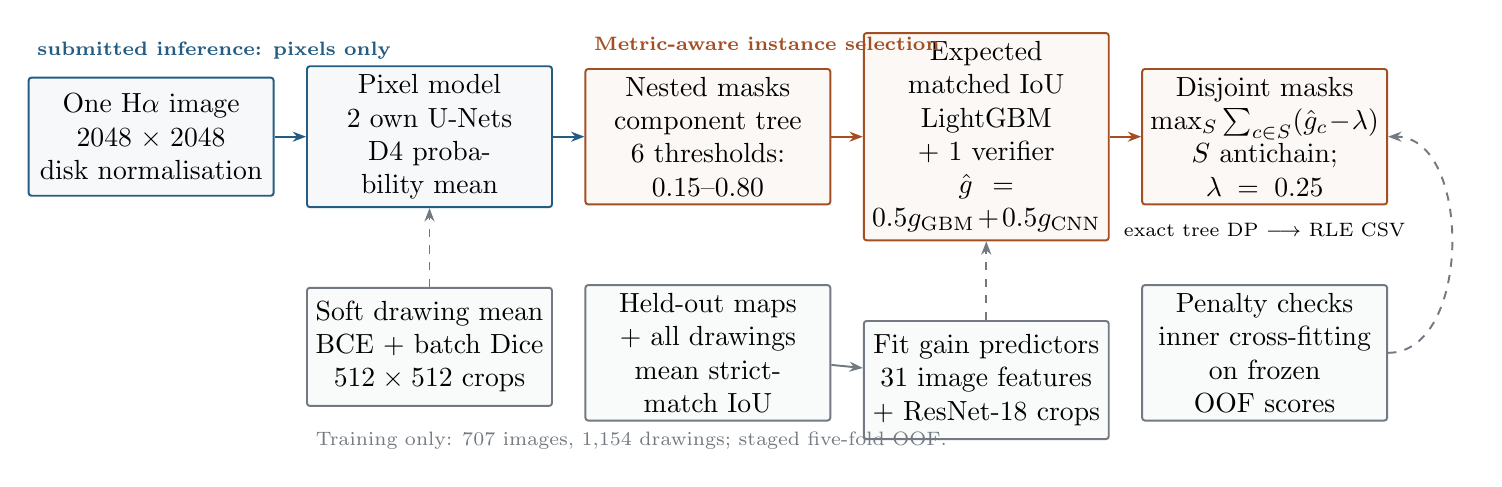
\begin{tikzpicture}[
  node distance=4mm and 4mm,
  box/.style={draw=#1,line width=0.7pt,rounded corners=1pt,align=center,
    minimum height=15mm,text width=29mm,inner sep=3pt,fill=#1!4},
  arr/.style={-{Stealth[length=1.7mm]},line width=0.7pt,draw=#1},
  lab/.style={font=\scriptsize\bfseries,anchor=south west}
]
\node[box=pixel] (image) {One H$\alpha$ image\\$2048\times2048$\\disk normalisation};
\node[box=pixel,right=of image] (pixel) {Pixel model\\2 own U-Nets\\D4 probability mean};
\node[box=select,right=of pixel] (tree) {Nested masks\\component tree\\6 thresholds: 0.15--0.80};
\node[box=select,right=of tree] (gain) {Expected matched IoU\\LightGBM + 1 verifier\\$\hat g=0.5g_{\rm GBM}+0.5g_{\rm CNN}$};
\node[box=select,right=of gain] (dp) {Disjoint masks\\$\max_{S}\sum_{c\in S}(\hat g_c-\lambda)$\\$S$ antichain; $\lambda=0.25$};
\draw[arr=pixel] (image)--(pixel);
\draw[arr=pixel] (pixel)--(tree);
\draw[arr=select] (tree)--(gain);
\draw[arr=select] (gain)--(dp);
\node[font=\scriptsize,anchor=north] at ([yshift=-1mm]dp.south) {exact tree DP $\longrightarrow$ RLE CSV};
\node[box=train,below=10mm of pixel] (soft) {Soft drawing mean\\BCE + batch Dice\\$512\times512$ crops};
\node[box=train,below=10mm of tree] (targets) {Held-out maps\\+ all drawings\\mean strict-match IoU};
\node[box=train,below=10mm of gain] (fit) {Fit gain predictors\\31 image features\\+ ResNet-18 crops};
\node[box=train,below=10mm of dp] (penalty) {Penalty checks\\inner cross-fitting\\on frozen OOF scores};
\draw[arr=train,dashed] (soft)--(pixel);
\draw[arr=train] (targets)--(fit);
\draw[arr=train,dashed] (fit)--(gain);
\draw[arr=train,dashed] (penalty.east) to[out=0,in=0] (dp.east);
\node[lab,text=pixel] at ([yshift=1mm]image.north west) {submitted inference: pixels only};
\node[lab,text=select] at ([yshift=1mm]tree.north west) {Metric-aware instance selection};
\node[align=left,font=\scriptsize,text=train,anchor=north west]
  at ([yshift=-2mm]soft.south west) {Training only: 707 images, 1,154 drawings; staged five-fold OOF.};
\end{tikzpicture}
\end{document}
